% =====================================================================================
% Caratterizzazione dell'ambiente RFI di Medicina in banda L (incluso da pipeline.tex)
% =====================================================================================
\FloatBarrier
\section{L'ambiente RFI di Medicina in banda L}
\label{sec:rfienv}

Questa sezione riassume ciò che le analisi precedenti dicono dell'ambiente di interferenze e del rumore del sistema,
indipendentemente dalla pipeline. Si basa su due osservazioni con lo stesso setup
(\SIrange{1382.25}{1446.25}{\mega\hertz}, 256 canali da \SI{0.25}{\mega\hertz}, \SI{16}{\micro\second}, 8 bit):
\begin{itemize}
  \item \file{ag278m_mc_no0004} (\SI{1199}{\second}, campo di un transiente, Sez.~\ref{sec:results} e seguenti);
  \item \file{ag293m_mc_no0001} (\SI{179}{\second}, puntamento su B0329+54).
\end{itemize}
I filterbank sono già limitati a \SI{64}{\mega\hertz}: la banda del ricevitore è più ampia, ma è stata tagliata a
monte a causa di RFI persistente molto forte. Anche la tabella delle prestazioni dell'antenna indica a
\SI{1.4}{\giga\hertz} una banda utile ridotta ($2\times\SI{80}{\mega\hertz}$) per le interferenze.

% -------------------------------------------------------------------------------------
\subsection{Tipi di interferenza}

\begin{table}[ht]
\centering
\caption{Inventario delle interferenze nelle due osservazioni, dai censimenti (\file{rfi_survey.py}) e dai
riassunti degli step della pipeline.}
\label{tab:rfienv}
\small
\begin{tabular}{p{3.3cm}p{5.6cm}p{5.6cm}}
\toprule
 & \file{ag278m_mc_no0004} (\SI{1199}{\second}) & \file{ag293m_mc_no0001} (\SI{179}{\second}) \\
\midrule
Canali inutilizzabili (maschera dello step 1) & 8: 121--127 (\SIrange{1414.4}{1415.9}{\mega\hertz}) e 185
  (\SI{1399.9}{\mega\hertz}) & 20: 0, 85, 140--145, 185, 200--205, 240--244 (gruppi a \num{1409.9}--\num{1411.1},
  \num{1394.9}--\num{1396.1}, \num{1385.1}--\SI{1386.1}{\mega\hertz}), con curtosi anomala \\
Salti di guadagno a banda larga & 1366 (\SI{1.1}{\per\second}), più forti ai bordi della banda & 65
  (\SI{0.36}{\per\second}) \\
Rete elettrica & \SI{50.0000006}{\hertz} e 55 armoniche fino a \SI{30}{\kilo\hertz}; 45.8\% della varianza della serie a
  DM 0 & \SI{50.000004}{\hertz}, 21 armoniche \\
Radar & due sorgenti con periodo \SI{10.0}{\second}: A a banda intera, B nella metà bassa; passaggi di circa
  \SI{90}{\milli\second} con treni di impulsi da \SI{0.5}{\milli\second} ogni \SIrange{2}{3}{\milli\second}, fino a
  S/N 120 a DM 0 & presenti con la stessa struttura (es. \SIrange{0.91}{0.955}{\second}) \\
Impulsi periodici rettangolari & -- & periodo \SI{0.50334}{\second} (\SI{1.987}{\hertz}), larghi
  \SI{8.5}{\milli\second}, non dispersi, simultanei in tutti i canali, più forti nei canali bassi: 356 su 356 periodi
  \\
Emissione a banda stretta persistente & \SIrange{1436}{1440}{\mega\hertz}, \SIrange{1420}{1422}{\mega\hertz},
  \SIrange{1387}{1390}{\mega\hertz}, variabile su decine di secondi; impulsi brevi a \SIrange{1415}{1420}{\mega\hertz}
  & -- (non analizzata) \\
Eventi impulsivi a DM 0 (step 3) & 72747 (\SI{61}{\per\second}); 3.4\% dei dati sostituiti & 10381
  (\SI{58}{\per\second}); 3.2\% dei dati sostituiti \\
\bottomrule
\end{tabular}
\end{table}

Alcune osservazioni:
\begin{itemize}
  \item \textbf{Il tasso di eventi impulsivi a DM 0 è lo stesso nelle due osservazioni} (circa 60 al secondo), mentre
    canali cattivi e salti di guadagno cambiano molto. Gli impulsi sembrano una caratteristica stabile del sito; canali
    e guadagno dipendono dalla sessione.
  \item \textbf{Gli impulsi periodici a \SI{1.987}{\hertz}} di \file{ag293m} sono stati inizialmente scambiati per la
    pulsar. Lo spettro dinamico a DM 0 mostra però bordi di salita e discesa simultanei in tutti i canali, e dedispersi a
    DM 26.7 si inclinano: non sono dispersi. \ipotesi{La forma rettangolare e la periodicità rigorosa suggeriscono
    un'apparecchiatura che commuta periodicamente.}
  \item \textbf{I radar} sono il disturbo impulsivo più intenso. Nella ricerca di \file{ag278m} sono stati la principale
    sorgente di candidati spuri dopo lo step 1 (Tab.~\ref{tab:step3}).
\end{itemize}

% -------------------------------------------------------------------------------------
\subsection{Rumore correlato tra i canali}

In entrambe le osservazioni il rumore della serie a DM 0 a banda intera è molto superiore a quello atteso per canali
indipendenti, e cresce con la scala di tempo: un rumore comune a tutti i canali e ``rosso''.
\begin{center}
\small
\begin{tabular}{lcc}
\toprule
 & \file{ag278m_mc_no0004} & \file{ag293m_mc_no0001} \\
\midrule
Rumore a DM 0 / atteso, su \SI{1}{\milli\second} (dopo lo step 3) & 4.4 (pilota: 4.47) & 4.74 \\
Idem su \SI{16}{\milli\second} / \SI{65}{\milli\second} & 11 / 17 & -- \\
Correlazione residua tra metà alta e metà bassa della banda & 2.48 & 2.52 \\
Accoppiamento dei canali al modo comune (mediana; 10°--90° percentile) & 0.75 (0.36--1.70) & 0.71 (0.46--1.88) \\
\bottomrule
\end{tabular}
\end{center}
I valori sono quasi identici nelle due osservazioni: il rumore correlato è una proprietà stabile del sistema, non un
episodio. L'accoppiamento varia molto da canale a canale, e una parte della correlazione (la differenza tra le due metà
della banda) non è descritta da un solo modo comune.

% -------------------------------------------------------------------------------------
\subsection{Sensibilità: B0329+54}
\label{sec:b0329}

\paragraph{Prestazioni nominali.} Dal manuale dell'antenna (Tab.~5.2, a \ang{45} di elevazione): a
\SI{1.4}{\giga\hertz} $T_{\rm sys}=\SI{58}{\kelvin}$, $G=\SI{0.120}{\kelvin\per\jansky}$, efficienza 41\%, da cui
$\text{SEFD}=T_{\rm sys}/G\simeq\SI{483}{\jansky}$ per polarizzazione.

\paragraph{Metodo.} Il file \file{ag293m_mc_no0001} è stato ripiegato con \file{prepfold} al periodo
\SI{0.71452}{\second} e DM 26.76, 128 intervalli di fase, dopo ogni step della pipeline. L'S/N del profilo è misurato
come segnale integrato sui 6 intervalli dell'impulso (circa \SI{34}{\milli\second}) diviso il rumore robusto fuori
dall'impulso. Il $\chi^2$ di \file{prepfold} non è adatto al confronto: presuppone rumore bianco ed è gonfiato dal
rumore correlato (da 1438 nell'originale a 4.9 dopo lo step 4, ma per la riduzione del rumore, non del segnale).

\paragraph{Rumore radiometrico.} Dopo lo step 1 ogni canale ha rumore $\sigma=8$ conteggi, quindi il rumore bianco
atteso per intervallo di fase è $8\sqrt{N_{\rm canali}}\sqrt{N_{\rm campioni/bin}}=8\sqrt{236}\sqrt{86400}\simeq
\num{3.6e4}$ conteggi. Il rumore misurato fuori impulso è 6.7--7.2 volte questo valore negli step 1--3 e 1.4 volte
dopo lo step 4. Rispetto al rumore radiometrico la pulsar ha S/N\,$\simeq$\,172; rispetto a quello reale circa 25.

\begin{table}[ht]
\centering
\caption{B0329+54 dopo ogni step: S/N del profilo rispetto al rumore reale, rapporto tra rumore reale e radiometrico,
segnale integrato rispetto allo step 2.}
\label{tab:b0329}
\small
\begin{tabular}{lcccc}
\toprule
 & S/N del picco & S/N integrato & rumore / radiometrico & segnale / step 2 \\
\midrule
originale & 19.4 & 24.9 & -- & -- \\
step 1 & 19.1 & 23.7 & 7.2 & 1.00 \\
step 2 & 20.8 & 25.7 & 6.7 & 1.00 \\
step 3 & 16.9 & 21.7 & 7.3 & 0.92 \\
step 4 & 12.6 & 8.8 & 1.4 & 0.07 \\
\bottomrule
\end{tabular}
\end{table}

\paragraph{Flusso e SEFD.} Con l'equazione del radiometro,
\begin{equation}
S_{\rm media}=\frac{\text{SEFD}}{\sqrt{n_{\rm pol}\,\Delta\nu\,\tau_{\rm bin}}}\cdot
\frac{\text{S/N}_{\rm int}\sqrt{N_{\rm on}}}{N_{\rm bin}},
\end{equation}
con $\Delta\nu=\SI{59}{\mega\hertz}$ (canali attivi), $\tau_{\rm bin}=\SI{176.9}{\second}/128$, $N_{\rm on}=6$,
$N_{\rm bin}=128$ e lo S/N radiometrico, si ottiene $S_{\rm media}\simeq \text{SEFD}\times\num{2.6e-4}$ per
$n_{\rm pol}=2$ e $\text{SEFD}\times\num{3.7e-4}$ per $n_{\rm pol}=1$. Con la SEFD nominale:
\begin{center}
\small
\begin{tabular}{lccc}
\toprule
Polarizzazioni nel file & $S_{\rm media}$ misurato & rapporto con il catalogo ($\simeq\SI{203}{\milli\jansky}$) &
  S/N radiometrico atteso \\
\midrule
2 & $\simeq\SI{125}{\milli\jansky}$ & 0.62 & $\simeq280$ \\
1 & $\simeq\SI{175}{\milli\jansky}$ & 0.87 & $\simeq200$ \\
\bottomrule
\end{tabular}
\end{center}
Viceversa, il flusso di catalogo implica una SEFD effettiva di circa \SI{790}{\jansky} ($n_{\rm pol}=2$) o
\SI{560}{\jansky} ($n_{\rm pol}=1$). Le incertezze principali sono la scintillazione di B0329+54 in banda L (il flusso in
un dato giorno può discostarsi dal valore di catalogo del 30--50\%), l'elevazione (la tabella vale a \ang{45}), il
puntamento e il numero di polarizzazioni nel file, da confermare. \ipotesi{Il flusso di catalogo è citato a memoria
(ATNF, $S_{1400}$) e va verificato.}

\paragraph{Lettura.}
\begin{itemize}
  \item \textbf{La SEFD del sistema è compatibile con quella nominale} entro un fattore 1.2--1.6, cioè entro le
    incertezze: non c'è indicazione di un ricevitore che renda meno del previsto. Il taglio a \SI{64}{\mega\hertz} non
    cambia la SEFD (grandezza per unità di banda) ma solo $\Delta\nu$. \ipotesi{L'RFI forte fuori dalla banda
    conservata potrebbe però aumentare $T_{\rm sys}$ nei canali rimasti, per compressione o intermodulazione
    nell'elettronica o per i fianchi dei filtri: un aumento della SEFD effettiva di questo tipo non è distinguibile, con
    questi dati, dalla scintillazione.}
  \item \textbf{La perdita di sensibilità viene dal rumore correlato}, non dalla SEFD: il profilo ripiegato è circa 7
    volte più rumoroso del limite radiometrico (S/N 25 invece di circa 170 in \SI{177}{\second}). Lo stesso fattore si
    ritrova, sulle scale dei millisecondi, nella serie a DM 0 di entrambe le osservazioni e nel pilota della campagna
    di completezza.
  \item \textbf{Effetto della pipeline sulla pulsar} (Tab.~\ref{tab:b0329}, Fig.~\ref{fig:b0329}): gli step 1 e 2 non
    perdono segnale; lo step 3 ne conserva il 92\% (rimuove alcuni impulsi singoli brillanti, visti a DM 0); lo step 4 ne
    conserva solo il 7\% e deforma il profilo. L'impulso di B0329+54 (circa \SIrange{6}{7}{\milli\second}) è più largo
    del proprio sweep su \SI{64}{\mega\hertz} (\SI{5}{\milli\second}), quindi in ogni istante è presente in quasi tutti i
    canali e viene sottratto come modo comune: è il limite larghezza/sweep previsto (Sez.~\ref{sec:step4}), qui confermato
    su dati reali.
\end{itemize}

\begin{figure}[ht]
\centering
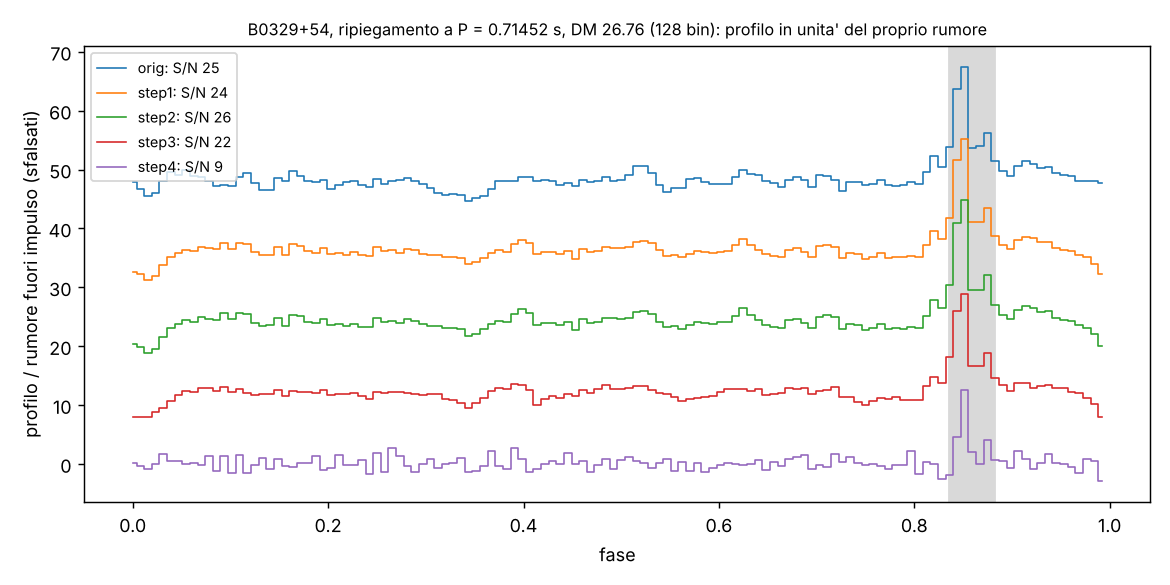
\includegraphics[width=0.85\textwidth]{fig/pipeline/B0329_profiles.png}
\caption{Profili di B0329+54 (\file{ag293m_mc_no0001}, \SI{177}{\second}, 128 intervalli) nel file originale e dopo
ogni step, ciascuno in unità del proprio rumore fuori impulso e sfalsati in verticale. In grigio la finestra
dell'impulso usata per l'S/N.}
\label{fig:b0329}
\end{figure}

\begin{figure}[ht]
\centering
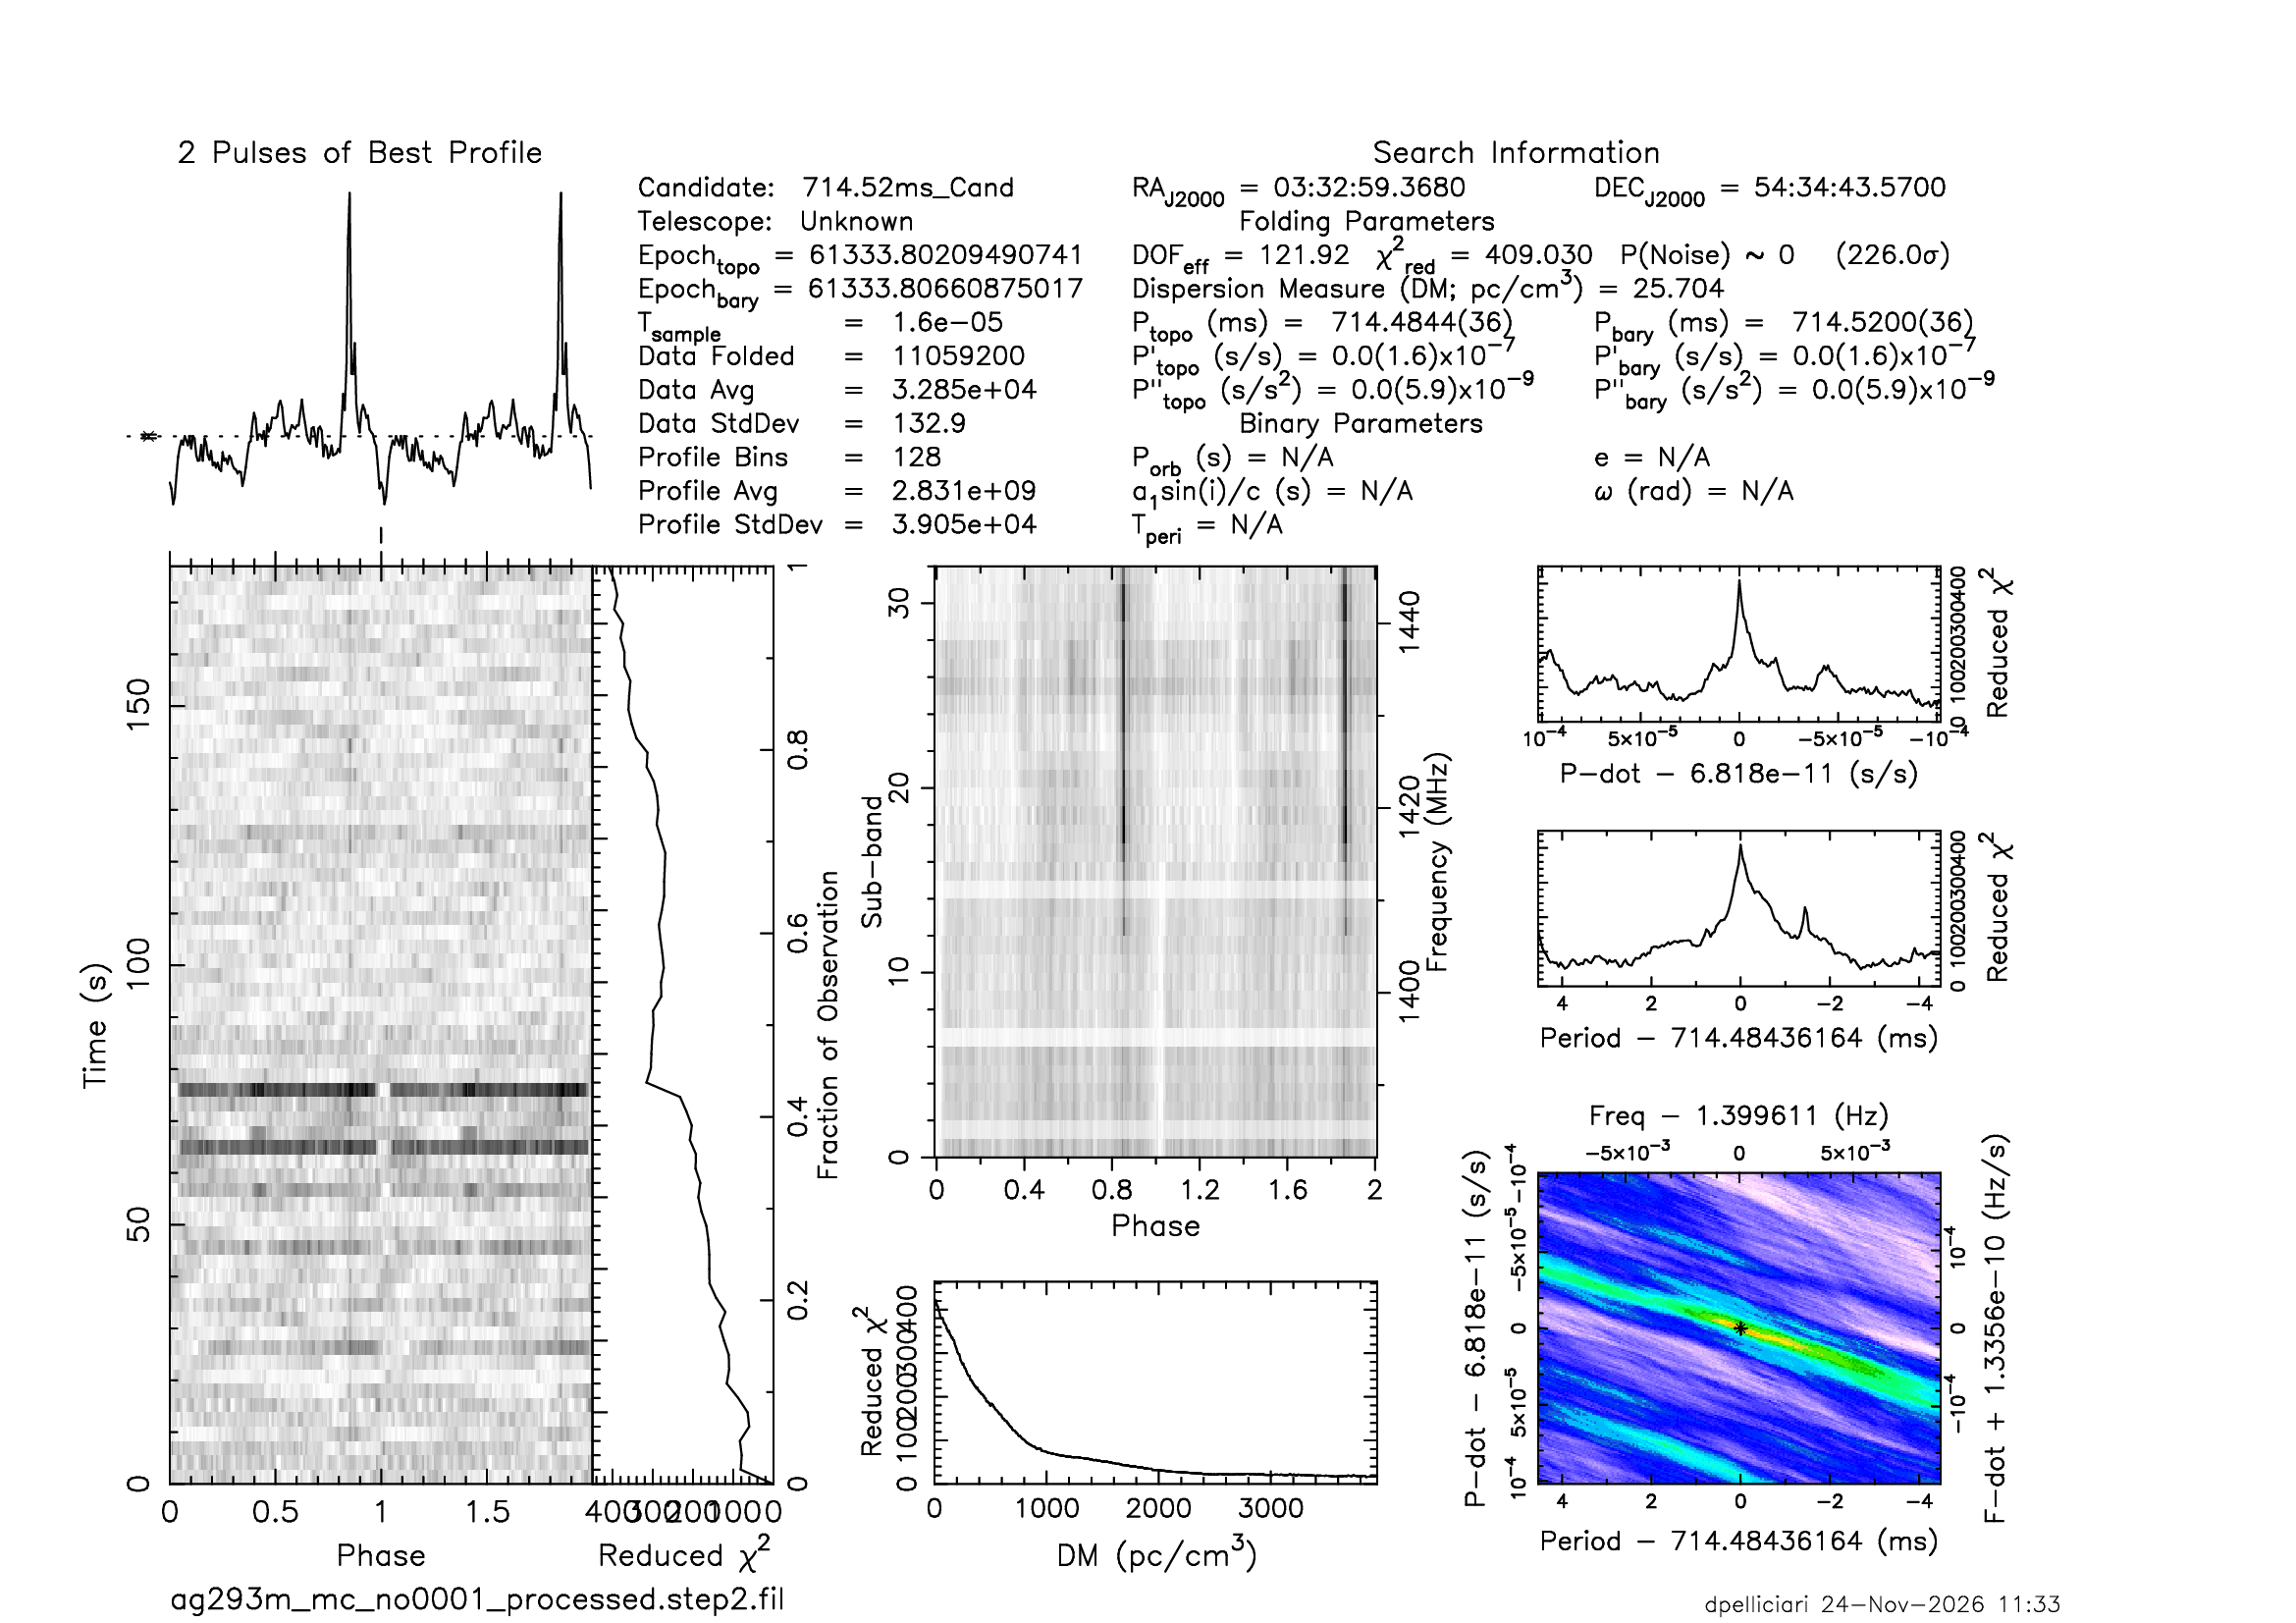
\includegraphics[width=0.95\textwidth]{fig/pipeline/B0329_prepfold_step2.png}
\caption{Ripiegamento di \file{prepfold} dopo lo step 2 (B0329+54, $P=\SI{0.71452}{\second}$, DM 26.76): profilo,
fase--tempo, fase--sottobanda e curve di $\chi^2$. Il $\chi^2$ riportato è gonfiato dal rumore correlato e non misura la
forza della pulsar (vedi testo).}
\label{fig:b0329pfd}
\end{figure}

% -------------------------------------------------------------------------------------
\subsection{Indicazioni per il sistema}
\begin{enumerate}
  \item Il guadagno in sensibilità più grande non verrebbe dalla pulizia a valle, ma dall'eliminazione del
    \textbf{rumore correlato tra i canali}, che costa un fattore circa 7 sui segnali impulsivi e ripiegati. Le possibili
    origini da verificare: elettronica di conversione, digitalizzazione, un controllo automatico del guadagno o
    un'altra regolazione a valle (compatibile con i salti di guadagno a intervalli di circa \SI{1}{\second}),
    interferenze a banda larga.
  \item Confermare con i tecnici: numero di polarizzazioni nei filterbank, elevazione durante le osservazioni, presenza
    di regolazioni automatiche del guadagno.
  \item Identificare le sorgenti locali: i due radar con periodo di \SI{10}{\second}, l'apparecchiatura a
    \SI{1.987}{\hertz}, l'emissione persistente a \SIrange{1436}{1440}{\mega\hertz} e \SIrange{1420}{1422}{\mega\hertz}.
  \item Ripetere la misura su B0329+54 in più giorni, per separare la scintillazione da eventuali variazioni del
    sistema, e con un calibratore nella stessa sessione per una SEFD assoluta.
\end{enumerate}
